\documentclass{scrartcl}
\usepackage{dominatrix}
\usepackage{tikz}
\usetikzlibrary{shapes,arrows,positioning}
\tikzstyle{kinect} = [rectangle, draw, text width=4em, rounded corners, text centered, minimum height=4em]
\tikzstyle{server} = [circle, draw, text width=4em, text centered, minimum height=4em]
\tikzstyle{workstation} = [rectangle, draw, text width=4em, rounded corners, text centered, minimum height=2em]
\tikzstyle{computer} = [rectangle, draw, text width=4em, rounded corners, text centered, minimum height=2em]
\tikzstyle{line} = [draw, -latex']
\subject{CS 4999 Independent Research}
\title{Midterm Report}
\subtitle{Cornell University Program for Computer Graphics}
\author{Lim Mingjie, Kenneth (\href{mailto:kl545@cornell.edu}{kl545}), Leart Albert Ulaj (\href{mailto:lau8@cornell.edu}{lau8})}
\date{\today}
\begin{document}
  \maketitle
  \begin{abstract}
    Lorem Ipsum
  \end{abstract}
  \tableofcontents
  \newpage
  \section{Foreword}
    This paper accompanies software code and documentation hosted on a private version control server, to which access is available on request.
  \section{Overview}
    Microsoft's new Kinect for Windows, released under the Kinect for Windows Development (K4WDev) Program\footnote{\url{http://www.microsoft.com/en-us/kinectforwindowsdev/newdevkit.aspx}} incorporates a time-of-flight (TOF) laser for depth-sensing at an effective range of 1--15 feet (0.3--4.5 meters). The higher level of precision and increased range of the TOF laser (compared to the older Kinect, which uses a pseudo-random infrared dot pattern) makes the new Kinect a suitable candidate for gesture-recognition applications in:\begin{inparaenum}[(1)]
      \item environments where it is not always possible for the user to be situated in front of the sensor such that depth detection is optimized;
      \item environments where the user may be one of multiple bodies in the sensor's field-of-view (FOV), of which it is difficult to disambiguate the actions and gestures of the other non-participatory bodies and the number of bodies far exceeds the number that can be tracked by the Kinect; and
      \item environments which are not well-lit.
    \end{inparaenum}

    Although the Kinect's target field of application is video gaming, the robustness of its 3-D capture data has encouraged both research at the academic level, and independent projects of varying scale at the amateur/enthusiast level. Most approaches to gesture-based interfaces, however, rely on joint-tracking rather than recognition. A set of parameters, e.g.~velocities and accelerations, or user-defined point clouds in the sensor's FOV are specified for the purpose of localizing and tracking movement. For example, a number of applications have been developed using USC's Flexible Action and Articulated Skeleton Toolkit (FAAST) and SigmaRD's SigmaNIL Hand Recognition Framework, among others. Although many approaches have been shown to work well in scripted scenarios, one would expect difficulties deploying these approaches in real-world scenarios due to differences in users' body parameters and movement styles.

    In this paper, we describe the use of a supervised constraint-based algorithm for robust gesture detection using the new Kinect. The algorithm is simple, extensible, and computationally efficient. We also describe the use of temporal averaging methods in the design of a user interface that consumes gestural data from the Kinect. Lastly, we contextualize this software ecosystem in the use of classroom (or instructional facility) design as an example of a real-world deployment scenario.
  \section{Project Specifications}
    \begin{figure}[ht!]
      \centering
      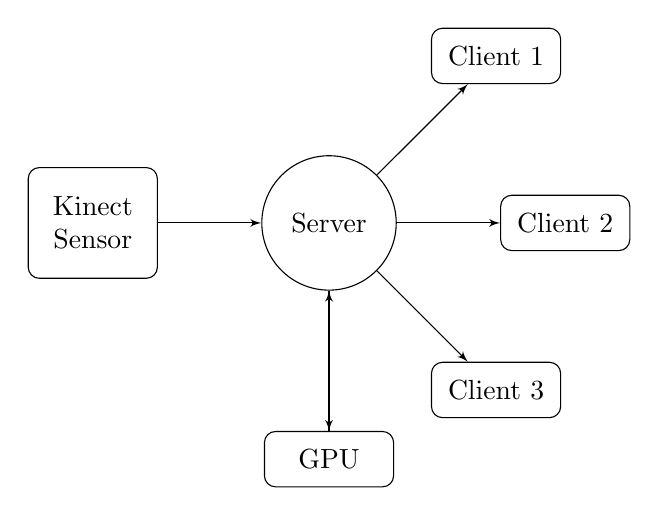
\begin{tikzpicture}[node distance = 3cm, auto]
        \node [kinect] (kinect) {Kinect Sensor};
        \node [server, right of=kinect] (server) {Server};
        \node [workstation, below of=server] (gpu) {GPU};
        \node [computer, right of=server] (client2) {Client 2};
        \node [computer, above right of=server] (client1) {Client 1};
        \node [computer, below right of=server] (client3) {Client 3};

        \path [line] (kinect) -- (server);
        \path [line] (server) -- (gpu);
        \path [line] (gpu) -- (server);
        \path [line] (server) -- (client1);
        \path [line] (server) -- (client2);
        \path [line] (server) -- (client3);
      \end{tikzpicture}
      \caption{Software infrastructure event flowchart depicting the Kinect sensor interfacing with three clients via the server.\label{fig:pipeline}}
    \end{figure}
    The software is conceptualized as a hybrid client capable of supporting multiple connections. The back-end is written in a low-level language that interfaces directly with the Kinect (via the Microsoft Kinect API) and uses the workstation's graphical processing unit (GPU) to convert raw sensor data into well-formed intermediate output. The intention is to offload processor-intensive computations to the workstation and stream the output to the front-end, which is a modular, lightweight application with little to no dependencies. The front-end consumes the output and renders graphical content to the user's display. Figure~\ref{fig:pipeline} depicts the flow of data from the Kinect sensor to the server, where it is interpreted before being piped to connected user clients.

    Establishing the software as a dichotomy of a front-end and back-end allows for the front-end to be adapted for different applications, treating the output from the server as a black-boxed ``bag-of-features''. In addition, since the Microsoft Kinect API is still under development, new changes can be slipstreamed into the back-end without further modification to the rest of the software infrastructure.
    \subsection{Hardware}
      We utilize the new Kinect sensor, provided to the Cornell Program of Computer Graphics (PCG) by Microsoft under the K4WDev program. Interaction with the application was done on an 82-inch Perceptive Pixels Inc. (PPI) touchscreen display at HD resolution ($1920 \times 1080$). Testing was performed on a secondary, 52-inch PPI touchscreen display at 4K resolution ($3840 \times 2160$).

      % TODO: Describe classroom layout, Kinect positioning and use of tracking tripod mount: Soloshot
    \subsection{Back-End}
      % TODO: Describe C# formulation, use of Fleck WS server
    \subsection{Front-End}
      Content schema and human interaction feedback were rendered in real-time in a modern web browser. The application leverages the HTML5 WebSockets API to connect to the back-end, then renders incoming data on a GPU-accelerated HTML canvas layer overlaid on the application user interface. Serving the application via a web interface eliminates the need for users to install any software on their devices (since all assets can be hosted on a remote server) and allows for multiple (remote) connection instances without additional infrastructure overhead.

      % TODO: Describe application UI
  \section{Road-map}
    \renewcommand{\thesubsection}{\Roman{subsection}}
    \subsection{Core Functionality\label{phase1}}
      The Kinect SDK tracks 21 3-D joint coordinates of the human skeleton model in real-time (30 frames/sec), corresponding to the spatial location of a user in the Kinect sensor's FOV. This polling rate generates $21 \times 30 \times 3 = 1890$ real-valued skeleton model coordinates per second. In addition, the skeleton model is robust to variation in the shape and size of the human body, color and texture of clothing, and objects or surfaces in the background, thus we omit consideration for these variables (otherwise considered anomalies) in the design of our action model representation.

      \begin{figure}[ht!]
        \centering
        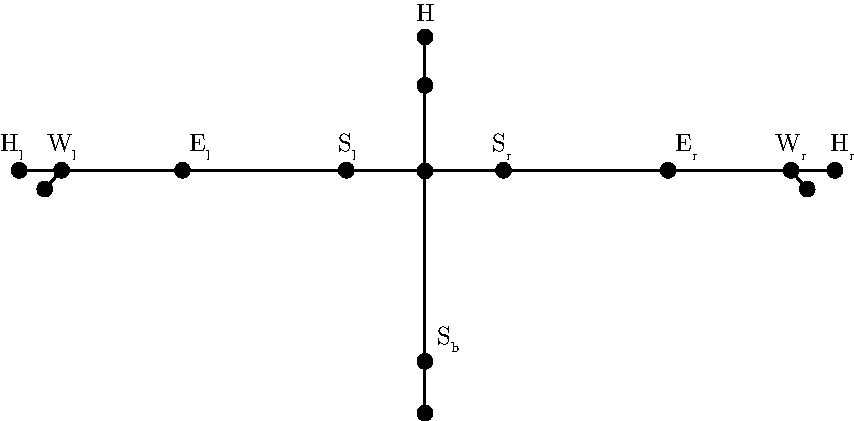
\includegraphics[width=0.75\textwidth]{img/Body}
        \caption{Partial joint nomenclature for the Kinect Skeleton Model, showing the top half of the body. Joints of interest are labeled, where $H$ corresponds to the head, $S_{\{ l,r \}}$ corresponds to the left or right shoulder, $E_{\{ l,r \}}$ corresponds to the left or right elbow, $W_{\{ l,r \}}$ corresponds to the left or right wrist, $H_{\{ l,r \}}$ corresponds to the left or right hand, and $S_b$ corresponds to the base of the spine.\label{fig:jointnomenclature}}
      \end{figure}
      Since our implementation is gesture-based, we begin by simplifying the skeleton model and focusing only on coordinates above the base of the spine. Specifically, the most pertinent joints are the left and right hand, left and right wrist, left and right elbow, and left and right shoulder. Figure~\ref{fig:jointnomenclature} assigns labels to these joints for ease of reference in subsequent discussions.
    \subsection{Establishing Coherence\label{phase2}}
      \subsubsection{Fleck WebSockets Server}
      \subsubsection{HTML5 WebSockets API}
      \subsection{Viewport Nomenclature}
    \subsection{Gestural Interaction\label{phase3}}
      As a simple nomenclature which we will build upon in this section, we classify gestures as either \emph{arm-level} gestures or \emph{hand-level} gestures. Eponymously, arm-level gestures involve the movement of the entire arm, such as pushing, pulling, or swiping actions. Hand-level gestures involve the movement of only the hand, such as expanding all fingers to show an open palm, clenching all fingers to form a fist, or extending a single finger to point in a direction.
      \subsection{Trigger Mechanism}
      In practice, gesture recognition must be applied to a finite data-set (e.g.~a video segment), in which the algorithm returns all statistically significant occurrences of a gesture within the data-set. In such cases, it is trivial to repeatedly expand a window of analysis to include frames before and after a suspected gesture component. However, it is not possible to deterministically identify a gesture when incoming data arrives as a stream, because the subsequent frames of data are unknown to the algorithm. We overcome this difficulty by constraining the initial set of permissible actions to the raising of the left or right hand above shoulder height. Specifically we define the constraints:
      \begin{align}
        x_{S_r} \leq x_{W_r} \leq x_{E_r} \\
        y_{S_r} \geq y_{W_r} \geq y_{E_r}
      \end{align}
      for detecting a raised right hand, and similarly:
      \begin{align}
        x_{S_l} \leq x_{W_l} \leq x_{E_l} \\
        y_{S_l} \geq y_{W_l} \geq y_{E_l}
      \end{align}
      for detecting a raised left hand.
      \subsubsection{Cursor Manipulation}
      \subsubsection{Hand States}
      \subsubsection{Pulling and Pushing}
      \subsubsection{Swiping}
      % TODO: Describe types of gestures -- arm level and hand level
    \subsection{Content Development\label{phase4}}
      % TODO: Describe ways of representing content
    \subsection{Testing and Robustness Evaluation\label{phase5}}
    \emph{This section provides a speculative overview of work that may be conducted this area, and will be updated as more information becomes available.}
      % TODO: Describe use of Kinect Fusion/QUnit for front/back-end testing
    \subsection{User Recognition\label{phase6}}
      \emph{This section provides a speculative overview of work that may be conducted this area, and will be updated as more information becomes available.}
      % TODO: Describe use Kinect Audio Beam-forming/IR Facial Recognition for saliency and recognition
  \section{Deliverables}
    \subsection{27 January}
      % Literature Review and familiarization with Kinect API
    \subsection{24 February}
      Phase~\ref{phase1} is expected to be completed by this time.
    \subsection{31 March}
      Phase~\ref{phase2} is expected to be completed by this time.
    \subsection{28 April}
      Phases~\ref{phase3} and~\ref{phase4} is expected to be completed by this time.
    \subsection{End of Semester}
      Phase~\ref{phase5} is expected to be completed by this time. % Phase 6 exploration.
  \section{Extensions}
    % Gesture Learning using ML
  \section{Acknowledgments}
    The authors are indebted to Donald Greenberg, Joe Kider, John Decorato, and Jeremy Newlin for advice and assistance rendered throughout the course of the project. This work was supported by the Cornell Program of Computer Graphics.
\end{document}
